\chapter{Key Theoretical Tools}
\label{theory}

With an appreciation now of the significance of a non-zero eEDM measurement, we can turn our attention to the challenge of achieving such a precise measurement. Possibly the simplest experiment one could devise would be to place an electron in an electric field and measure the energy change of the electron associated with the eEDM interaction, as given in equation $\ref{dipole_energy}$. This approach, whilst simple, falls apart very quickly since a free electron in an electric field will rapidly accelerate, leaving very little time for a precise measurement. A quick calculation shows that with the typical upper limit achievable laboratory electric field of $100 \text{kVcm}^{-1}$ and an eEDM of $10^{-29}$ e cm, the current experimental upper limit, the energy shift associated with an eEDM aligned with the field would be ${\sim}10^{-24} $eV. Whilst trying to measure such a small change in energy, the experimenters would have to contend with the electron accelerating at $\sim 10^{18} \text{m s}^{-2}$, making this simple approach practically impossible.

Instead experiments have utilised atoms or molecules to confine the electrons (see section \ref{enhancement_factor_section}), as well as more sophisticated techniques such as optical pumping (see section \ref{optical_pumping}) and carefully tuned fields for achieving specific superposition states (see section \ref{pi_pulses}), in order to create interferometers capable of measurements approaching the BSM predicted eEDM. In this section these topics will be reviewed, allowing for a deeper understanding of the modern experiments discussed in section \ref{modern_experiments}.

\section{Electric Field Enhancement Factor}
\label{enhancement_factor_section}

One major potential issue with measuring the EDM of an electron trapped in an atom is the potential shielding of the atom. Since the atom will polarise in the electric field it will seek a state with zero internal electric field, resulting in no eEDM interaction. This view was first presented in 1963 and is known as Schiff's theorem \cite{Schiff_1963}.

Whilst the argument presented by Schiff is valid for a non-relativistic treatment, Sandars showed that the full eEDM interaction term, including relativistic corrections, will evade Schiff's theorem, resulting in a non-zero, or even enhanced eEDM interaction \cite{Sandars_1965}. A detailed explanation for this evasion is given by Commins et al \cite{Commins_2007}, where they show that the evasion arises from a Lorentz contraction of the eEDM in the lab frame.

The evasion and resulting relativistic interaction is typically described by an enhancement factor, R, defined as

\begin{equation} \label{enhancement_factor_definition}
    R = \frac{\mathbf{d}_{a}}{\mathbf{d}_e}.
\end{equation}

Sandars shows it scales approximately as

\begin{equation} \label{enhancement_factor_scaling}
    R \sim P Z^{3} \alpha^{2}
\end{equation}

where $P$ denotes the polarisability of the atom, $Z$ is the atomic number and $\alpha$ is the fine structure constant. This scaling indicates that a greater EDM interaction will be present in heavy atoms.

However, atoms with high atomic numbers also have low polarisabilities, therefore limiting the magnitude of the enhancement. On the other hand molecules show much greater polarisability, allowing them to produce much greater effective electric fields, even in relatively weak applied electric fields.

Due to this significant polarisability the effective electric fields for molecules cannot simply be characterised by a single enhancement factor, instead one needs to consider the form of the non-linear polarisation of this alignment. Therefore the effective electric field of a molecule is often characterised by the following equation,

\begin{equation}
    \mathbf{E}_{eff} = \mathbf{E}^{max}_{eff} \eta (\mathbf{E_{app}}) \hat{z}
    \label{molecule_effective_field}
\end{equation}

where we have chosen the field to be aligned parallel to the z axis. The polarisation factor, denoted by $\eta$, ranges from 0 to 1 and describes how the alignment of the molecule changes with respect to the applied field. Since the form of this polarisation factor varies for different molecules it is important to compare their enhancement factors at a specific electric field, in table \ref{tab:enhancement_factors} this is chosen to be $E_{app} = 10 k\text{V} \text{cm}^{-1}$.

\begin{table}[h]
    \centerline{
        \resizebox{15cm}{!}{
            \begin{tabular}{ c c c c }
                Atom/Molecule & Enhancement Factor, R & Effective Electric Field, $E_{eff}$ & Reference \\
                \hline
                Caesium, Cs & 124 & $1.2 \times 10^{5}$ & \cite{dzuba_2009} \\
                Sodium, Na & 0.3 & $3.3 \times 10^{3}$ & \cite{dzuba_2009} \\
                Thallium, Tl & 582 & $5.8 \times 10^{5}$ & \cite{dzuba_2009} \\
                Ytterbium Fluoride, YbF & $2.6 \times 10^6$ & $2.6 \times 10^{10}$ & \cite{Mosyagin_1998} \\
                Thorium Monoxide, ThO & $10.4 \times 10^6$ & $10.4 \times 10^{10}$ & \cite{Meyer_2008} \\
            \end{tabular}
        }
    }
    \caption{\label{tab:enhancement_factors} Enhancement factors of atoms and molecules previously used or proposed for electron EDM experiments. The molecular enhancement factors and effective electric fields are evaluated at an applied electric field of $E_{app} = 10 k\text{V} \text{cm}^{-1}$.}
\end{table}

\section{Atomic energy structure}
\label{atomic_energy_structure}

Atomic energy level structure is key to the atomic beam experimental approach, therefore it is worth providing some background theory on this topic. The entire atomic Hamiltonian, up to hyperfine structure is given in equation \eqref{hamiltonian_to_hyperfine}.

\begin{equation} \label{hamiltonian_to_hyperfine}
    H = H_{0} + V_{Coulomb} \underbrace{- \frac{p^4}{8m^3c^2} + H_{SO} + H_{Darwin}}_\textup{Fine Structure} + \underbrace{H_{Zeeman}}_\textup{Hyperfine Structure} + H_{EDM}
\end{equation}

The key interaction in the subsequent atomic beam experiments lies in the hyperfine structure and the EDM interaction. Hyperfine structure arises from electromagnetic multipole moments of the nucleus interacting with the with the magnetic field induced by the orbital motion of the electron and it's spin. When including hyperfine structure the Hamiltonian becomes degenerate unless we consider the diagonal basis of the total spin, F, defined in equation \eqref{total_spin}.

\begin{equation} \label{total_spin}
    \textbf{F} = \textbf{I} + \textbf{J}
\end{equation}

where $\textbf{I}$ is the nuclear spin and $\textbf{J}$ is the total angular momentum.
 
A popular choice of atom for the atomic beam experiment has been Thallium, this is because it is the heaviest stable atom with one valence electron, giving it an enhancement factor of $R \simeq -585$ \cite{Liu_1992}. The valence electron of Thallium lies in the $6^2P_{1/2}$ ground state, for which $J = 1/2$ and $I = 1/2$, hence the valence electron can take $F = \{0, 1\}$. This implies four different F hyperfine sublevels as the $F = 1$ level has a multiplicity of $2F + 1$.

\section{Optical Pumping}
\label{optical_pumping}

Optical pumping is a commonly used technique for creating order in the distribution of electronic states in an ensemble of atoms. As the name suggests an optical field, such as a laser, is tuned to pump specific transitions and with specific polarisations it can select for specific sub-levels of the excited state. To determine the probability of these transitions we first define the interaction Hamiltonian to be the dipole interaction between the laser and the atom, given in equation \ref{interaction_hamiltonian}. Note that we assume the atom and laser are polarised along the z-axis.

\begin{equation} \label{interaction_hamiltonian}
    \hat{H}_{int} =  - \hat{\mathbf{d}} \cdot \mathbf{E} =  - \hat{d}_z E_{z} \cos({\omega t})
\end{equation}

The transition probabilities are calculated from the overlap of all possible hyperfine states, this can be performed using the Wigner-Eckhart theorem, as seen in equation \ref{transition_probability}.

\begin{equation} \label{transition_probability}
    \braket{F',m_F'|\hat{d}_z|F,m_F} = \braket{F,m_F,1,0|F',m_F'} \braket{F'||d||F}
\end{equation}

For the case optical pumping tuned to the $6^2P_{1/2} \rightarrow 6^2S_{1/2}$ transition the Clebsch-Gordon coefficients on the right hand side of equation \ref{transition_probability} will be non-zero for the excitations shown in solid lines in figure \ref{fig:optical_pumping_scheme}:

\begin{figure}
    \centerline{
        % Resize it to 5cm wide.
        \resizebox{10cm}{!}{
            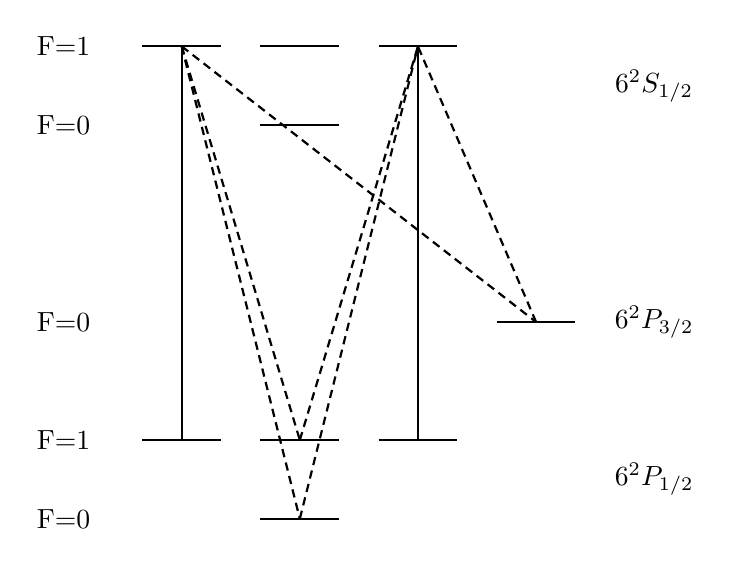
\begin{tikzpicture}[
              scale=0.5,
              level/.style={thick},
              decay/.style={thick,densely dashed},
              driven/.style={thick},
              classical/.style={thin,double,<->,shorten >=4pt,shorten <=4pt,>=stealth}
            ]
            % Level: 7S1/2
            \draw[level] (2cm,-2cm) -- (4cm,-2cm);
            \draw[level] (5cm,-2cm) -- (7cm,-2cm);
            \draw[level] (8cm,-2cm) -- (10cm,-2cm);
            \node at (0cm, -2cm) {F=1};

            \draw[level] (5cm,-4cm) -- (7cm,-4cm);
            \node at (0cm, -4cm) {F=0};
            
            \node at (15cm, -3cm) {$6^2S_{1/2}$};
            
            % Level: 6P3/2
            \draw[level] (11cm,-9cm) -- (13cm,-9cm);
            \node at (0cm, -9cm) {F=0};
            \node at (15cm, -9cm) {$6^2P_{3/2}$};

            % Level: 6P1/2
            \draw[level] (2cm,-12cm) -- (4cm,-12cm);
            \draw[level] (5cm,-12cm) -- (7cm,-12cm);
            \draw[level] (8cm,-12cm) -- (10cm,-12cm);
            \node at (0cm, -12cm) {F=1};

            \draw[level] (5cm,-14cm) -- (7cm,-14cm);
            \node at (0cm, -14cm) {F=0};
            
            \node at (15cm, -13cm) {$6^2P_{1/2}$};
            
            % Driven Transitions
            \draw[driven] (3cm,-12cm) -- (3cm,-2cm);
            \draw[driven] (9cm,-12cm) -- (9cm,-2cm);
            
            % Decays
            \draw[decay] (3cm,-2cm) -- (6cm,-12cm);
            \draw[decay] (6cm,-12cm) -- (9cm,-2cm);

            \draw[decay] (3cm,-2cm) -- (6cm,-14cm);
            \draw[decay] (6cm,-14cm) -- (9cm,-2cm);

            \draw[decay] (3cm,-2cm) -- (12cm,-9cm);
            \draw[decay] (12cm,-9cm) -- (9cm,-2cm);
            
            \end{tikzpicture}
        }
    }
    \caption{Optical pumping of thallium for $m_F=0$ state selection, driven excitations are denoted by solid lines and spontaneous decays are denoted by dashed lines}
    \label{fig:optical_pumping_scheme}
\end{figure}

\section{\texorpdfstring{$\pi/2$}{pi/2} Pulses}
\label{pi_pulses}

The previously discussed state selection process of optical pumping can be used to start the experiment in a pure state. However, often it is a superposition state that is be used to measure interactions between an eEDM and an electric field. Experimentally this superposition state can be achieved by applying a specially tuned pulse, commonly referred to as a $\pi/2$ pulse. To understand this process we start by considering a Hamiltonian of the following form

\begin{equation}
    H = H_0 + H_{int}
\end{equation}

where the interaction Hamiltonian $H_{int}$ is defined in equation \ref{interaction_hamiltonian}.

An arbitrary three level system of states $\{| 0 \rangle, | 1 \rangle, | -1 \rangle\}$ can be represented in a basis of $\{| 0 \rangle, | + \rangle, | - \rangle\}$, where we define

\begin{equation}
    | + \rangle = \frac{1}{\sqrt{2}} ( | 1 \rangle + | - 1 \rangle )
\end{equation}

\begin{equation}
    | - \rangle = \frac{1}{\sqrt{2}} ( | 1 \rangle - | - 1 \rangle )
\end{equation}

In this basis our interaction Hamiltonian does not couple the ground state, $| 0 \rangle$, to the state $| - \rangle$ and therefore in this basis our system is reduced to a two level system. With this reduced two level system one can then follow the approach laid out in Ramsey's book "Molecular Beams" in the derivation of equation V.7 \cite{Ramsey_1956}, in which the time dependent Schrodinger equation is used, alongside orthogonality constraints, to yield the following propagator associated with the light-atom interaction

\begin{equation}
    \label{pulse_propagator}
    \Pi_{rf}(t) = \begin{pmatrix}
        \cos(\omega t) e^{i \frac{\omega}{2} t} & - \sin(\omega t) e^{i \frac{\omega}{2} t} & 0 \\
        - \sin(\omega t) e^{-i \frac{\omega}{2} t} & \cos(\omega t) e^{-i \frac{\omega}{2} t} & 0 \\
         0 & 0 & e^{-i \frac{\omega}{2} t} \\
    \end{pmatrix}
\end{equation}

where $\omega$ is the corresponding angular frequency of the driving field, which is taken to be on resonance with the energy gap between the ground and coherent superposition excited state, $| + \rangle$.

We can understand this propagator more clearly by inspecting two specific timings of the pulse, first lets choose $\omega t = \pi$,

\begin{equation}
    \Pi_{rf}(t=\frac{\pi}{\omega}) = \begin{pmatrix}
         -i & 0 & 0 \\
         0 & i & 0 \\
         0 & 0 & -i \\
    \end{pmatrix}.
\end{equation}

This pulse is referred to as a $\pi$ pulse, assuming the system is initially prepared in the ground state, for example through the optical pumping scheme discussed in the previous section, this pulse will rotate the state around the Bloch sphere, shown in figure \ref{fig:bloch_sphere}. Another common pulse is defined by $\omega t = \frac{\pi}{2}$, with the corresponding propagator

\begin{equation}
    \Pi_{rf}(t=\frac{\pi}{2 \omega}) = e^{-i \frac{\pi}{4}} \begin{pmatrix}
         0 & i & 0 \\
         - 1 & 0 & 0 \\
         0 & 0 & 1 \\
    \end{pmatrix}.
\end{equation}

For a more detailed discussion of this process, as well as the full propagator, including off resonance driving, please refer to \cite{Tarbutt_2009}.